\documentclass[xcolor=dvipsnames,xcolor=table]{beamer}

\newcommand{\itmspace}[0]{\hspace{2cm}}

\newcommand{\abr}[1]{\textsc{#1}}
\newcommand{\camelabr}[2]{{\small #1}{\textsc{#2}}}
\newcommand{\triviaqa}{\camelabr{Trivia}{qa}}
\newcommand{\squad}{\textsc{sq}{\small u}\textsc{ad}}
\newcommand{\nq}[0]{\abr{nq}}
\newcommand{\qb}[0]{\abr{qb}}


\newcommand*{\tcircle}[1]{\tikz[anchor=base,baseline=-2.5pt] \node[circle,fill=#1,scale=0.9] (X) {};}
\newcommand*{\tsquare}[1]{\tikz[anchor=base,baseline=-2.5pt] \node[fill=#1,scale=1.2] (X) {};}
\newcommand*{\tdiamond}[1]{\tikz[anchor=base,baseline=-2.5pt] \node[diamond,fill=#1,scale=0.7] (X) {};}
\newcommand*{\ttriangle}[1]{\tikz[anchor=base,baseline=-1.5pt] \node[regular polygon,regular polygon sides=3,fill=#1,scale=0.6] (X) {};}

\usepackage{tikz}
\usetikzlibrary{shapes.geometric}

\usepackage{multirow}
\usepackage{overpic}
\usepackage{booktabs}
\usepackage[dvipsnames,table]{xcolor}

\usetheme[
          showdate=false,                     % show the date on the title page
          alternativetitlepage=true,         % Use the fancy title page.
          titlepagelogo=general_figures/shell,              % Logo for the fir\
st page.
          ]{UMD}


          \newcommand{\citename}[1]{\small{#1}}

\newcommand{\danquote}[1]{

\begin{flushright}
\begin{overpic}[width=5.5cm,tics=10]{general_figures/speech_bubble}
	\put(10,30) { \parbox{4cm}{#1 }}
\end{overpic}

\includegraphics[width=1.5cm]{general_figures/milkman_dan}
\end{flushright}
}

\newcommand{\gfxt}[2]{
\begin{center}
	\includegraphics[width=#2\linewidth]{teaparty/figures/#1}
\end{center}
}


          
\newcommand{\fsi}[2]{
\begin{frame}[plain]
\vspace*{-1pt}
\makebox[\linewidth]{\includegraphics[width=\paperwidth]{#1}}
\begin{center}
#2
\end{center}
\end{frame}
}

\newenvironment{variableblock}[2]{%
  \setbeamercolor{block body}{#2}
  \begin{block}{#1}}{\end{block}}

\newcommand{\gfxq}[2]{
\begin{center}
	\includegraphics[width=#2\linewidth]{qb/#1}
\end{center}
}


\newcommand{\goodbad}[2]{

\begin{columns}

  \column{.5\linewidth}

\begin{variableblock}{Good}{bg=PineGreen,fg=white}
  #1
\end{variableblock}


  \column{.5\linewidth}

\begin{variableblock}{Bad}{bg=BrickRed,fg=white}
  #2
\end{variableblock}


\end{columns}

}


\title[HITL ML]{Interactive Topic Models}
\author{Jordan Boyd-Graber et al.}
\date{2020}

%gets rid of bottom navigation bars
\setbeamertemplate{footline}[frame number]{}

%gets rid of bottom navigation symbols
\setbeamertemplate{navigation symbols}{}

%gets rid of footer
%will override 'frame number' instruction above
%comment out to revert to previous/default definitions
\setbeamertemplate{footline}{}


\begin{document}


\frame{
\titlepage
\tiny
}

\begin{frame}

\begin{center}
\frametitle{What does a Topic Model do?}
From an \textbf<1>{input corpus} and number of topics \textbf<1>{$K$} $\rightarrow$ \textbf<2>{words to topics} \\
\only<1>{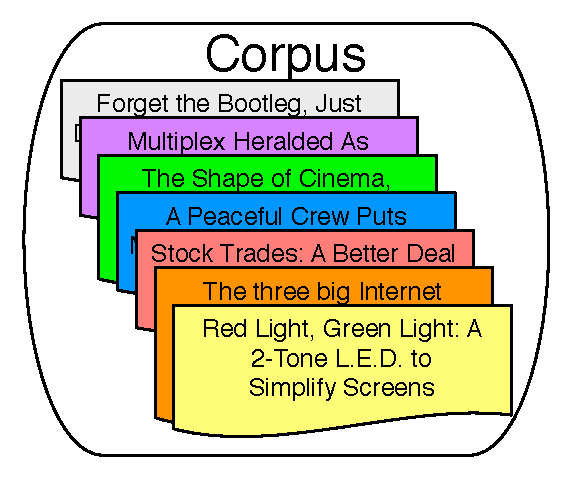
\includegraphics[width=0.6\linewidth]{reading_tea_leaves/figures/heldout_0} }
\only<2>{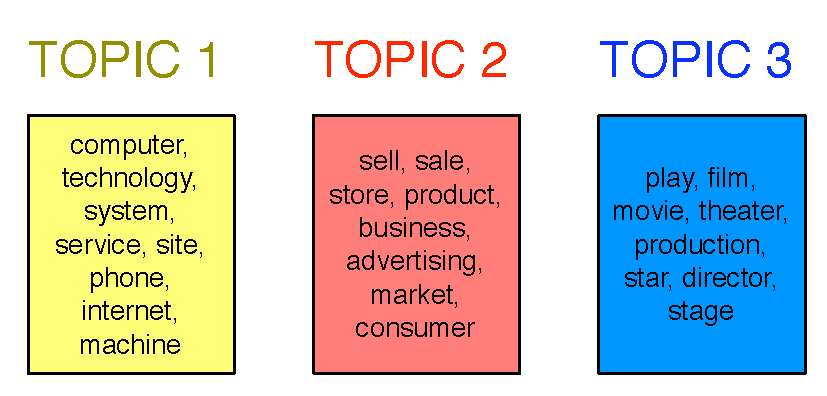
\includegraphics[width=0.9\linewidth]{reading_tea_leaves/figures/nyt_topics_wide}}
%\only<3>{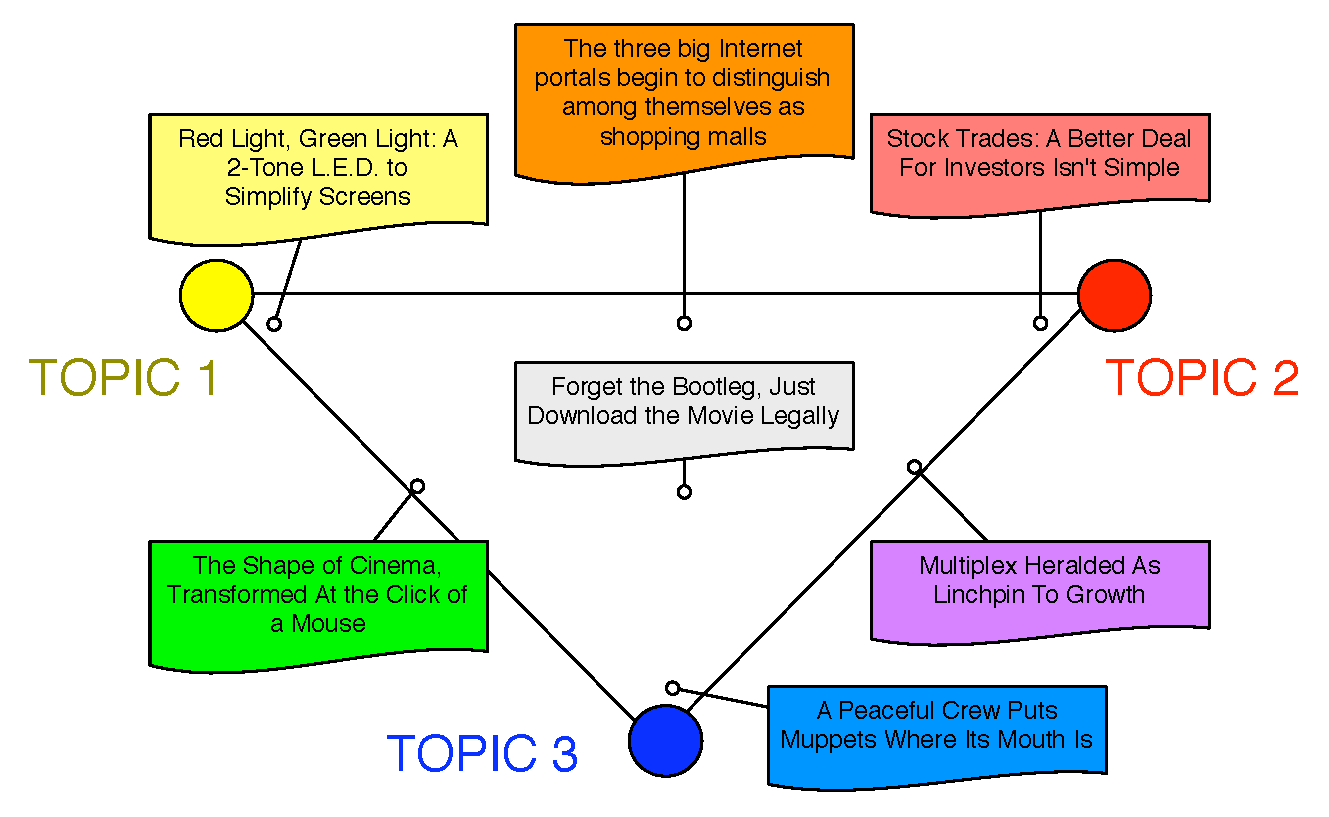
\includegraphics[width=0.9\linewidth]{topic_models/nyt_documents}}
\end{center}

\end{frame}


\begin{frame}{Evaluating Topic Models}

\begin{columns}

\column{.6\linewidth}
\begin{block}{ Reading Tea Leaves: How Humans Interpret Topic Models}
Jonathan Chang, Jordan Boyd-Graber, Chong Wang, Sean Gerrish, and David
M. Blei. Reading Tea Leaves: How Humans Interpret Topic Models. Neural
Information Processing Systems, 2009.
\end{block}

\column{.3\linewidth}
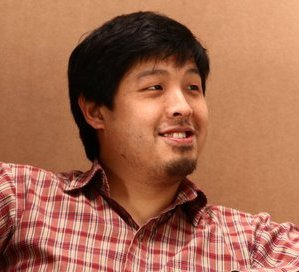
\includegraphics[width=.8\linewidth]{general_figures/jonathan}

\end{columns}

\end{frame}



\frame{
\frametitle{Evaluation}
\begin{center}
%\only<1>{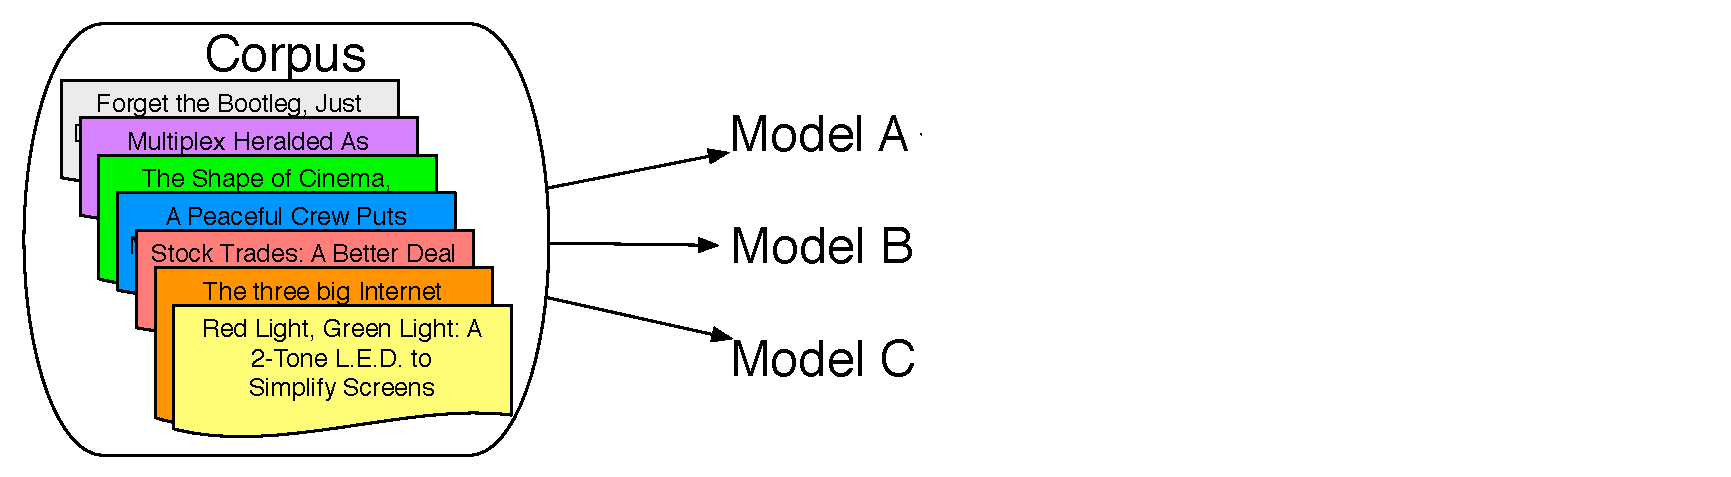
\includegraphics[width=0.9\linewidth]{reading_tea_leaves/figures/heldout_1} }
\only<1>{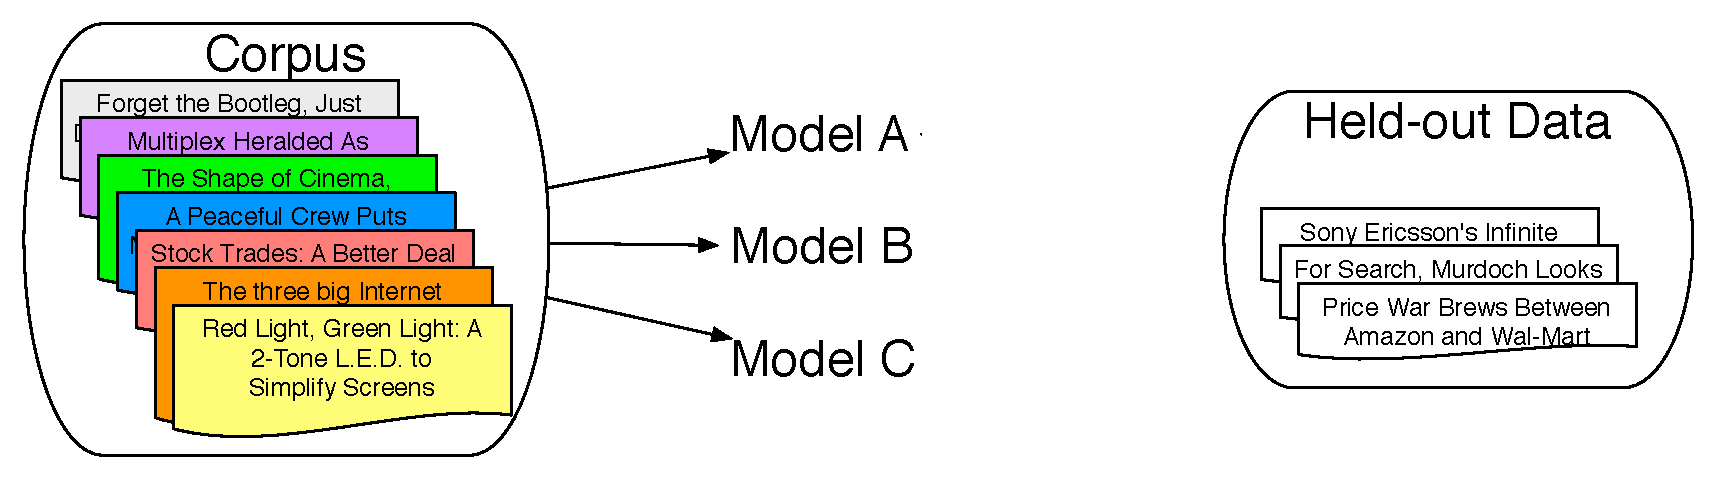
\includegraphics[width=\linewidth]{reading_tea_leaves/figures/heldout_2} }
%\only<3>{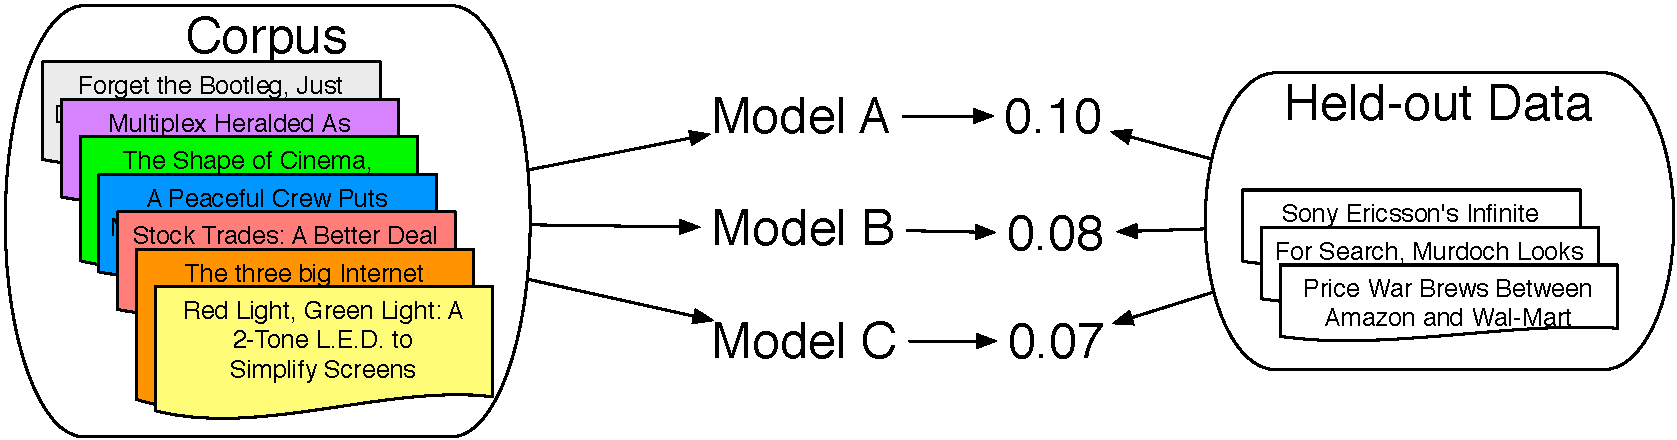
\includegraphics[width=\linewidth]{reading_tea_leaves/figures/heldout_3} }
\only<2>{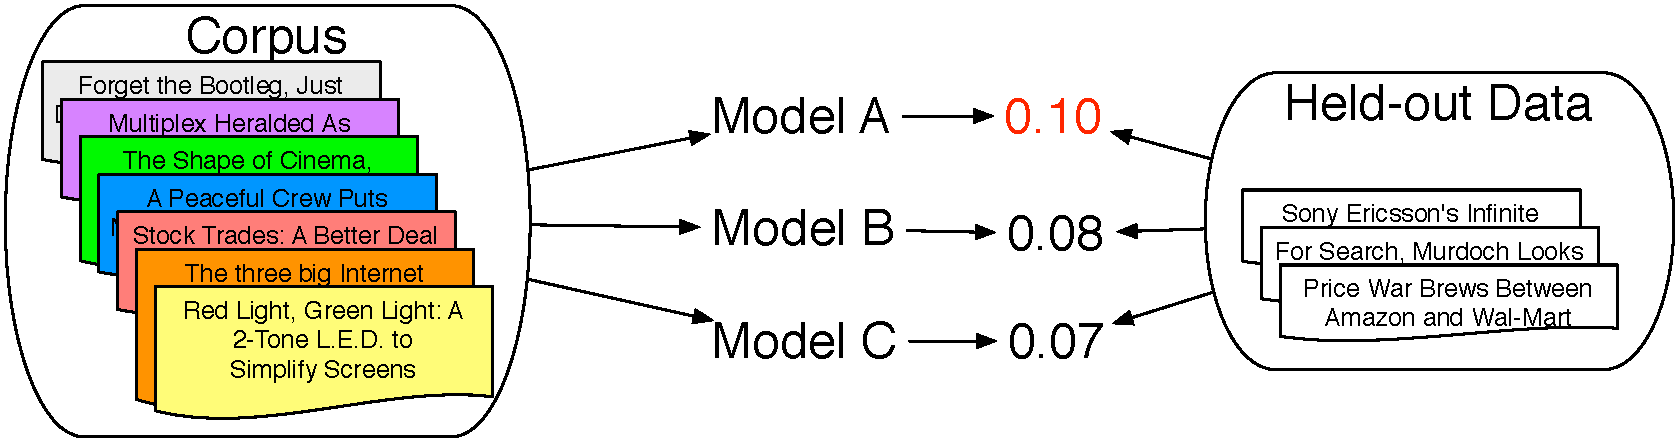
\includegraphics[width=\linewidth]{reading_tea_leaves/figures/heldout_4}  \\
	\large Measures predictive power (likelihood)}
\end{center}
}

\frame{
  \frametitle{Word Intrusion}

  \begin{itemize}
    \item Take the highest probability words from a topic

      \begin{block}{Original Topic}
        dog \\ cat \\ \only<2->{\alert<2->{apple} \\ } horse \\ pig \\ cow
      \end{block}

\only<2->{    \item \alert<2>{Intruder: high probability word from another topic}}
\pause
  \end{itemize}
}

\frame{
\frametitle{Interpretability and Likelihood}


\begin{center}
\only<1>{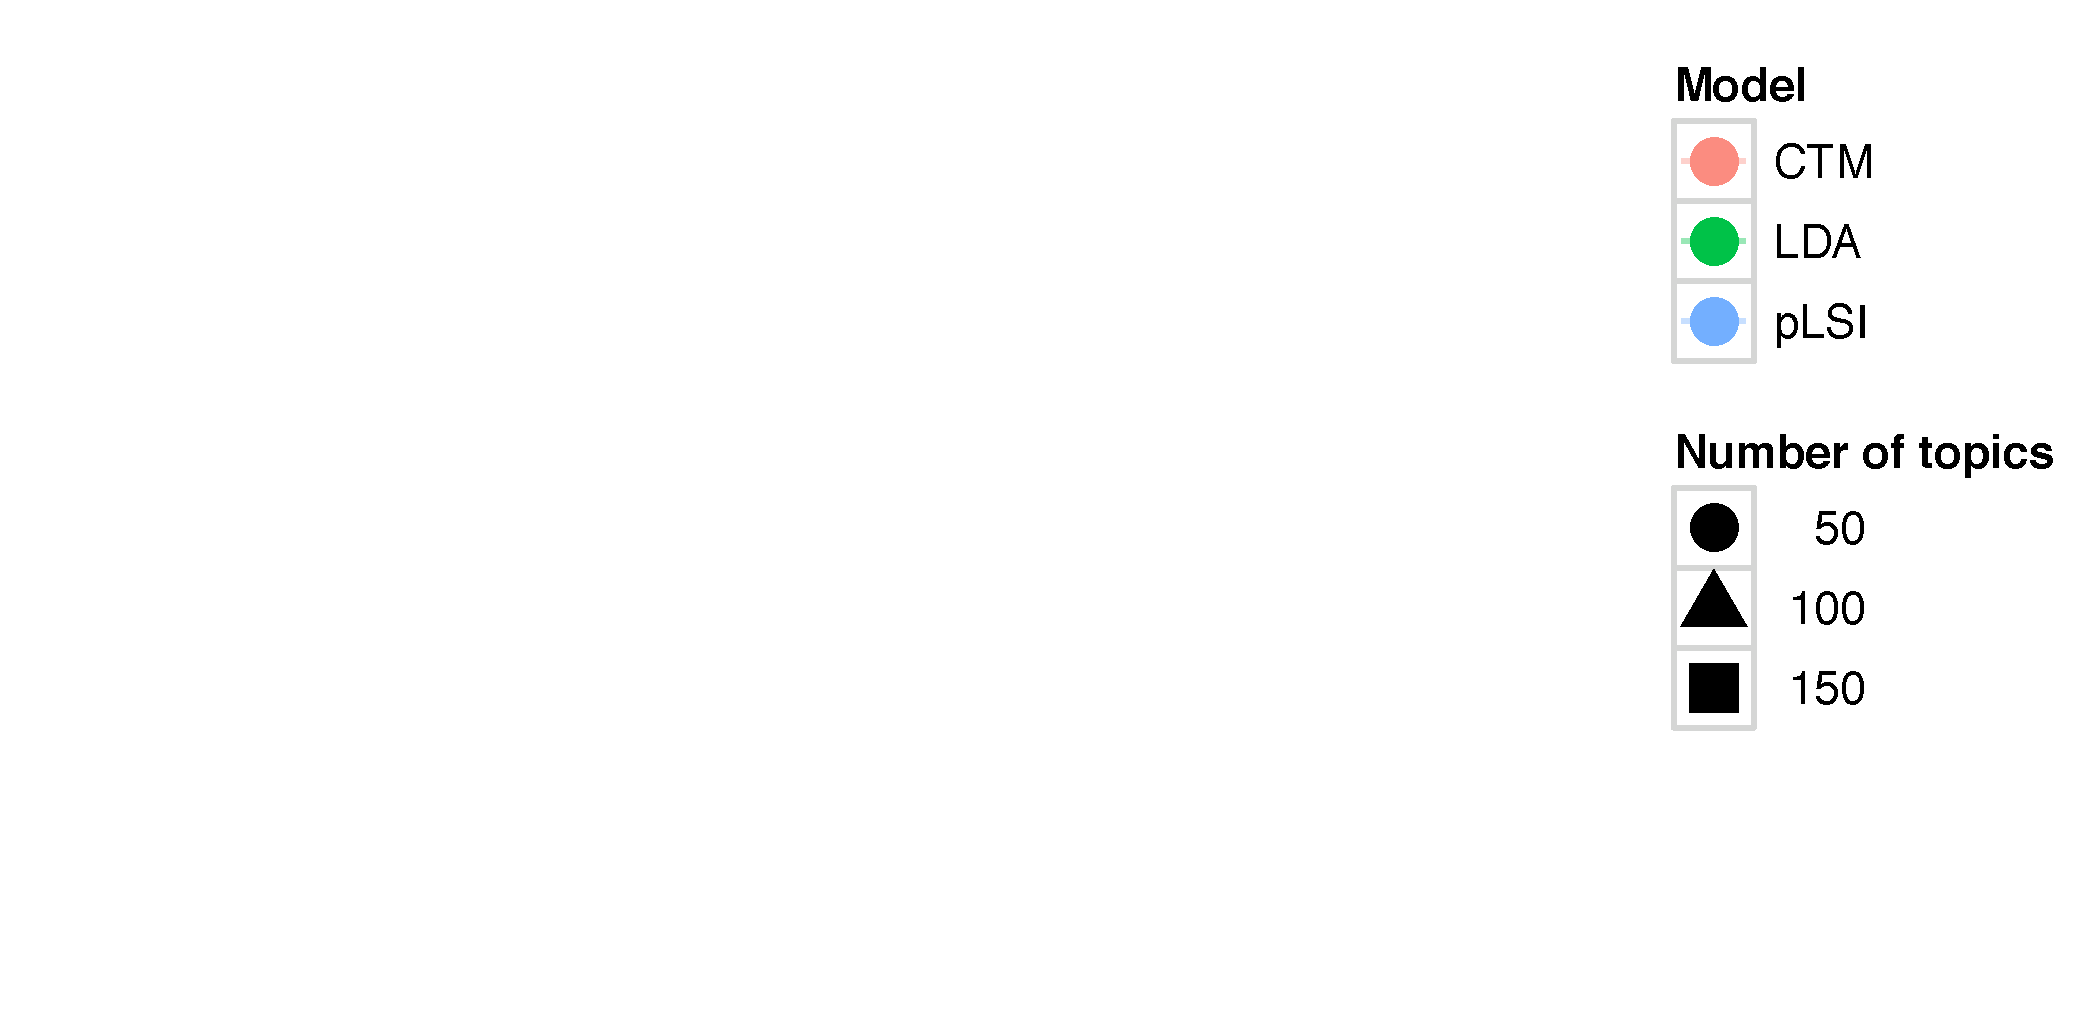
\includegraphics[width=.8\paperwidth]{reading_tea_leaves/figures/prec_ll_1}}
\only<2>{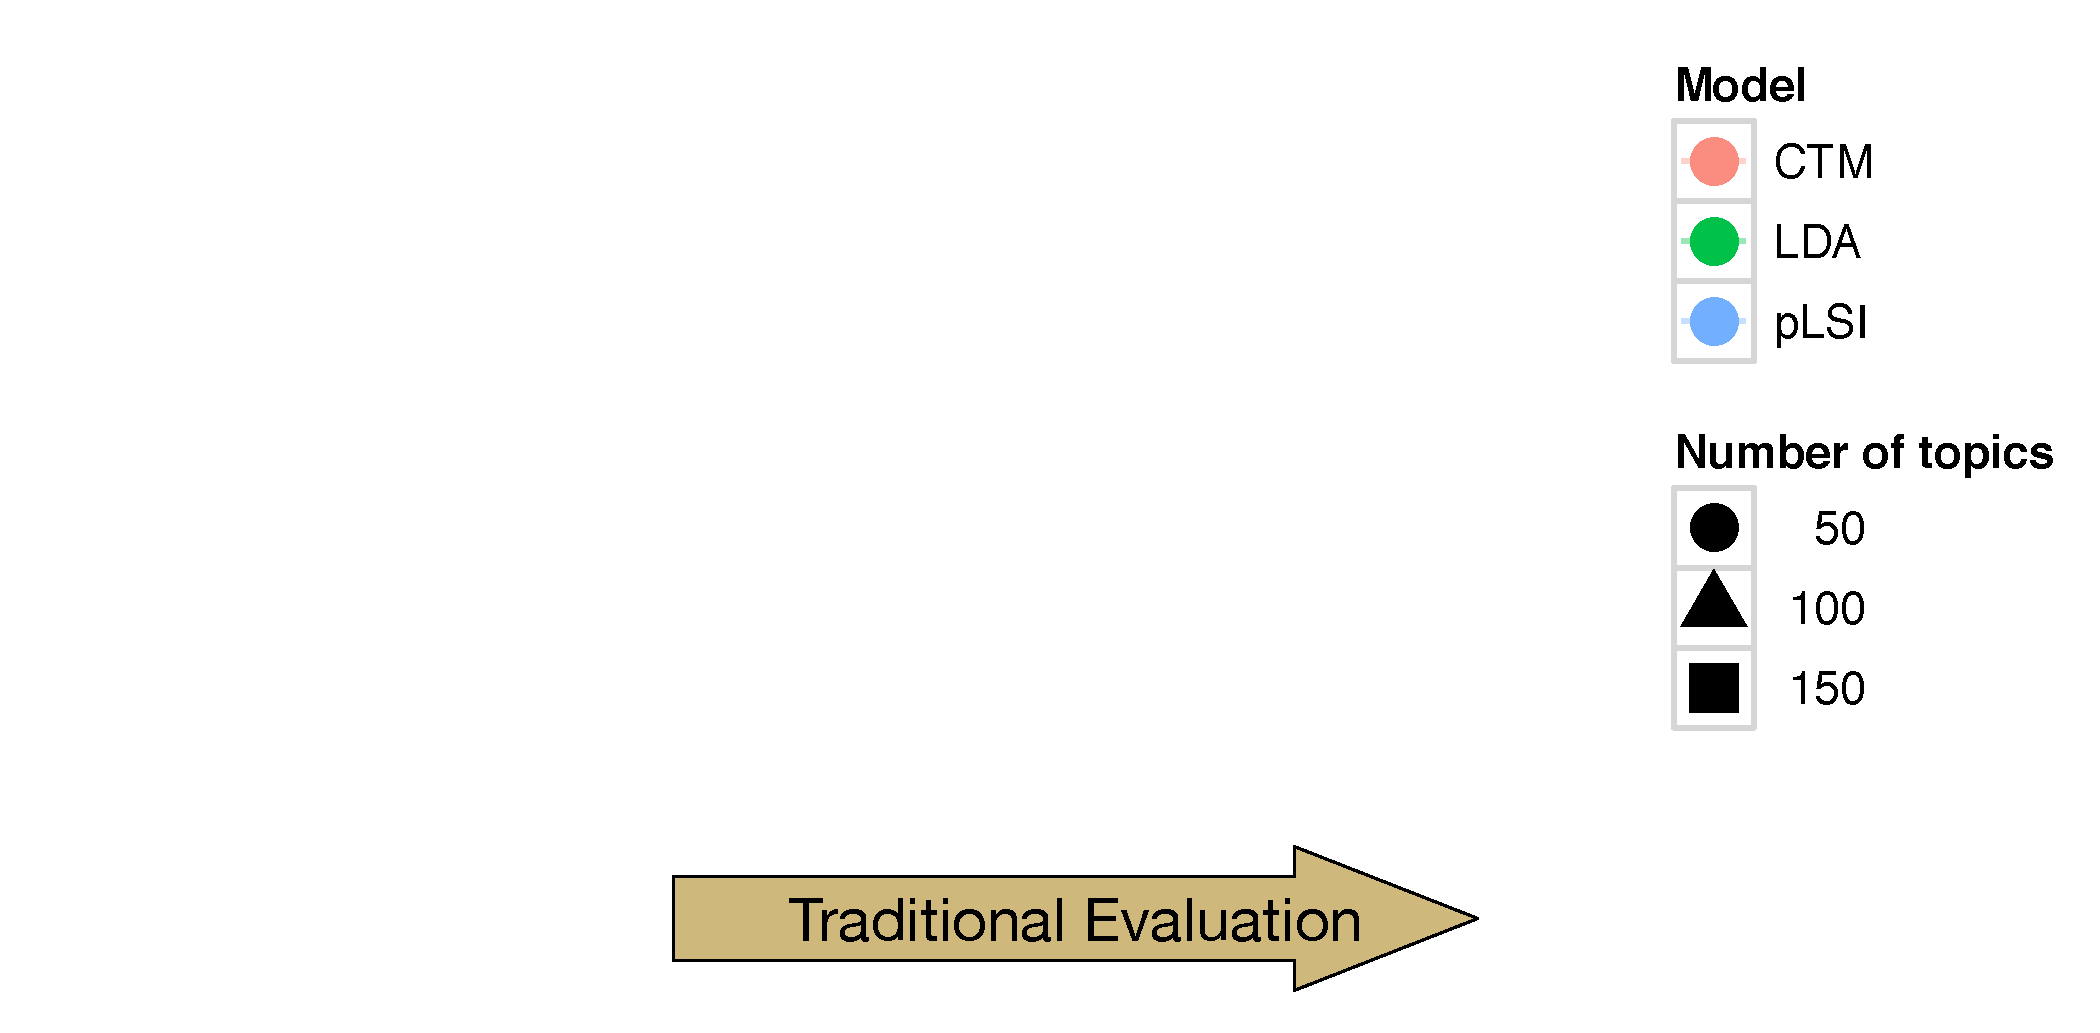
\includegraphics[width=.8\paperwidth]{reading_tea_leaves/figures/prec_ll_2}}
\only<3>{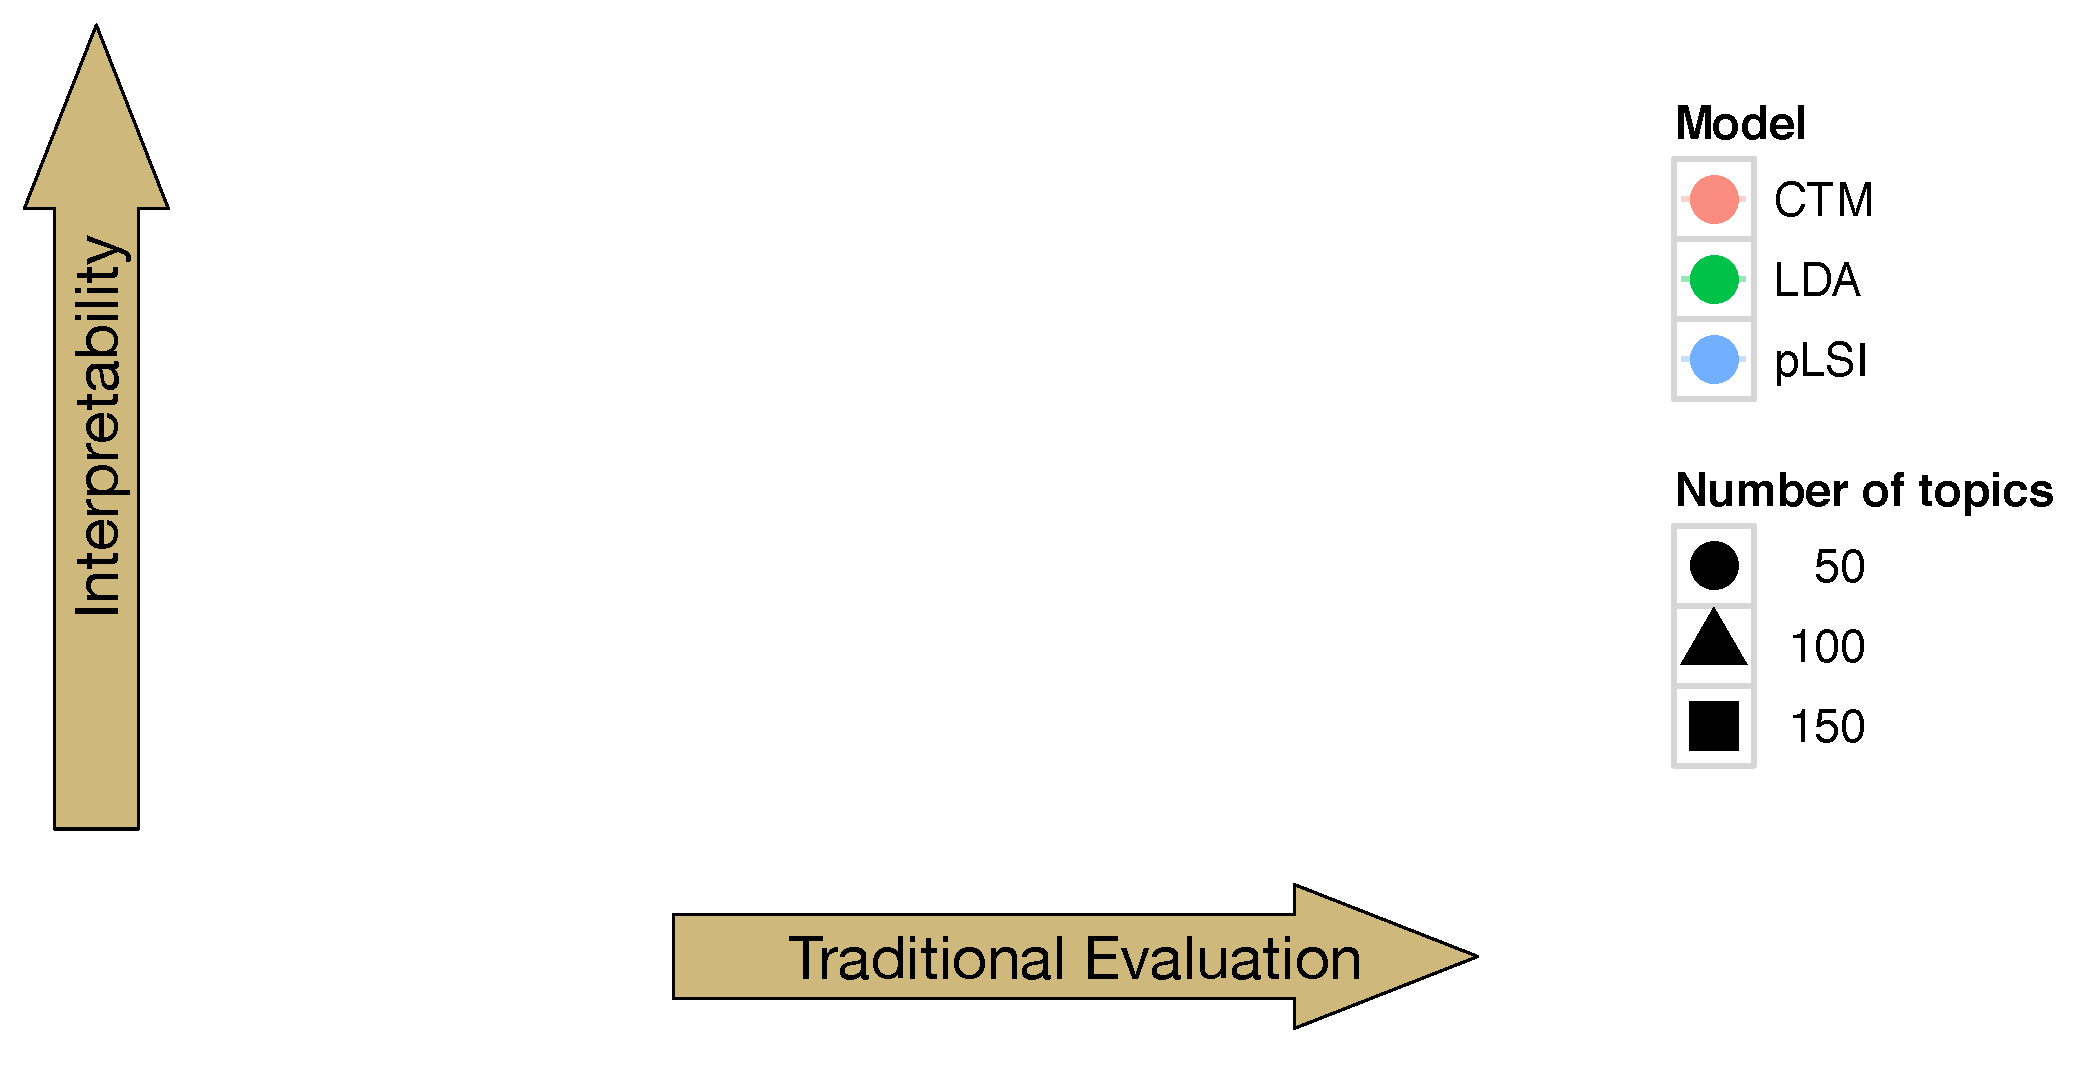
\includegraphics[width=.8\paperwidth]{reading_tea_leaves/figures/prec_ll_3}}
\only<4>{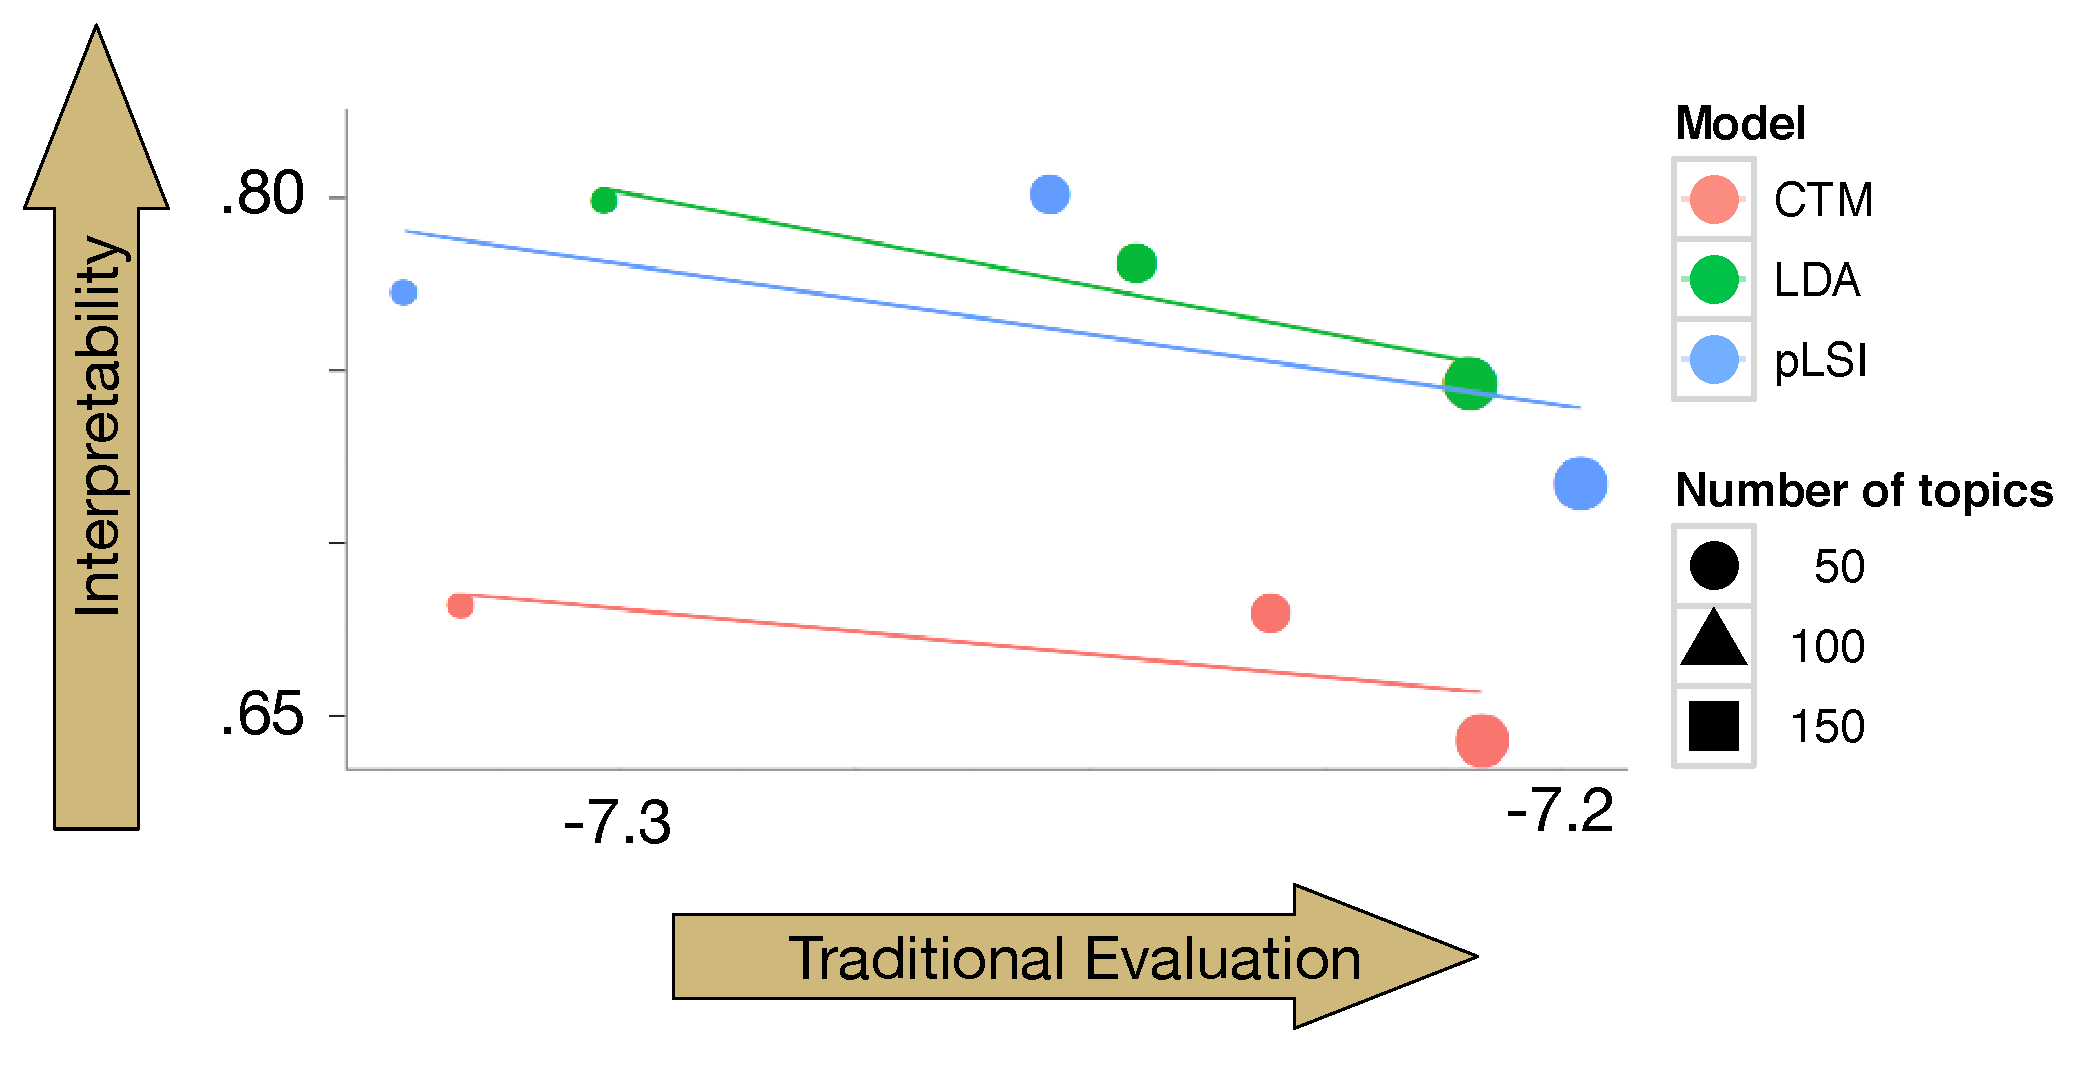
\includegraphics[width=.8\paperwidth]{reading_tea_leaves/figures/prec_ll_4}}
\only<4>{\\ Within a model, higher likelihood $\not =$ higher interpretability}
\end{center}
}





\begin{frame}
\frametitle{The Problem: User Perspective}

\begin{columns}

\column{.4\linewidth}
\begin{center}
\begin{tabular}{ccc}
& \only<2->{\itmspace}\color<2->{red}{bladder} & \\
& \only<3->{\hspace{-2cm}} \color<3->{blue}{spinal\_cord}  & \\
& \only<3->{\hspace{-2cm}} \color<3->{blue}{sci} & \\
& \only<3->{\hspace{-2cm}}\color<3->{blue}{spinal\_cord\_injury} & \\
& \only<3->{\hspace{-2cm}}\color<3->{blue}{spinal} & \\
& \only<2->{\itmspace}\color<2->{red}{urinary} & \\
& \only<2->{\itmspace}\color<2->{red}{urothelial} & \\
& \only<3->{\hspace{-2cm}}\color<3->{blue}{cervical} & \\
& injury & \\
& recovery & \\
& \only<2->{\itmspace}\color<2->{red}{urinary\_tract} & \\
& locomotor & \\
& \only<3->{\hspace{-2cm}}\color<3->{blue}{lumbar} & \\
\end{tabular}
\end{center}

\column{.6\linewidth}

\danquote{These words don't belong together!}

\end{columns}

\end{frame}


\frame{

\begin{columns}

\column{.5\linewidth}

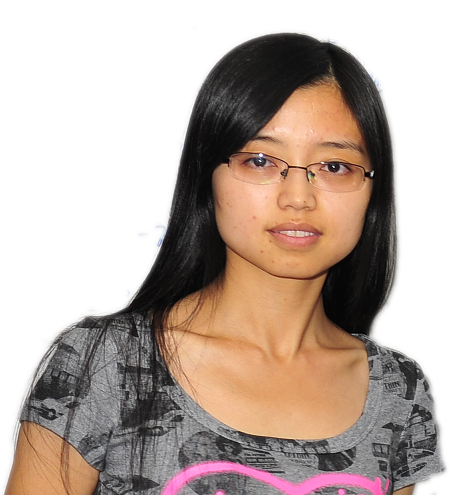
\includegraphics[width=.8\linewidth]{general_figures/yuening}

\column{.5\linewidth}

\begin{block}{Interactive Topic Modeling}
Yuening Hu, Jordan Boyd-Graber, and Brianna Satinoff.  Association for Computational Linguistics, 2011.
\end{block}


\end{columns}

}



\frame{
	\frametitle{How to fix it?}


	\only<1>{	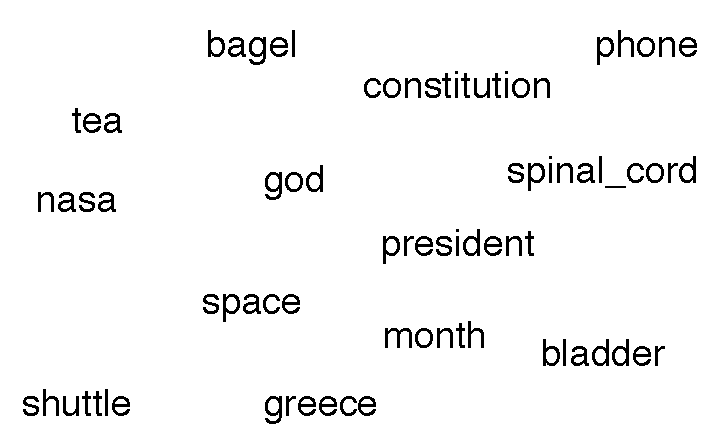
\includegraphics[width=\linewidth]{interactive_topic_models/constraints_1}     }
	\only<2>{	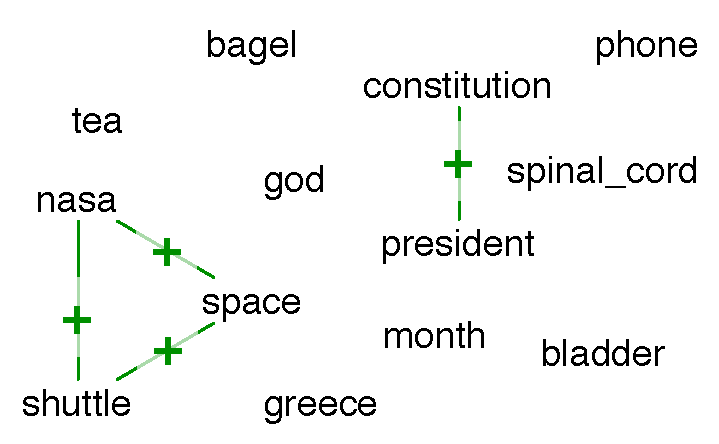
\includegraphics[width=\linewidth]{interactive_topic_models/constraints_2}     }
	\only<3>{	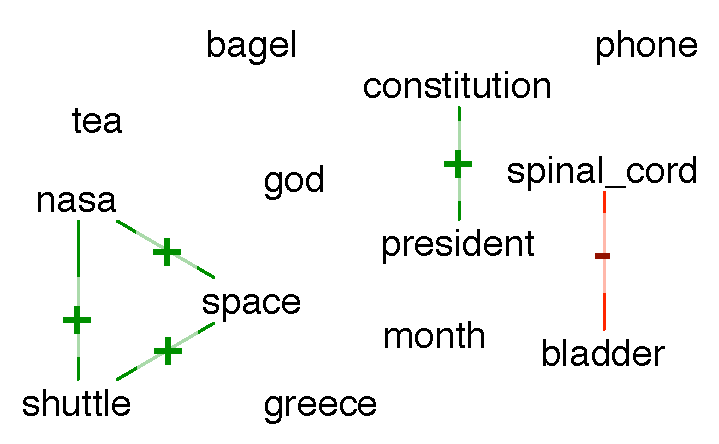
\includegraphics[width=\linewidth]{interactive_topic_models/constraints_3}     }


}


\providecommand{\tb}[1]{\parbox{0.8\linewidth}{ \tiny{ #1 }} \vspace{.2cm} }

\frame{

\vspace{-1cm}

\begin{columns}

\column{.5\linewidth}

\begin{tabular}{l*{2}{c}r}
	Topic & Before \\
\hline

\alert<2>{{\bf 1}} & \tb{ \alert<2>{election, yeltsin, russian, political, party, democratic, russia,
  president, democracy, boris, country, south, years, month, government, vote,
  since, leader, presidential, military} } \\

2 & \tb{new, york, city, state, mayor, budget, giuliani, council, cuomo, gov,
  plan, year, rudolph, dinkins, lead, need, governor, legislature, pataki,
  david} \\

3 & \tb{nuclear, arms, weapon, defense, treaty, missile, world, unite, yet,
  soviet, lead, secretary, would, control, korea, intelligence, test, nation,
  country, testing} \\

4 & \tb{president, bush, administration, clinton, american, force, reagan, war,
  unite, lead, economic, iraq, congress, america, iraqi, policy, aid,
  international, military, see} \\

& \vdots \\

\alert<2>{{\bf 20}} & \tb{\alert<2>{soviet, lead, gorbachev, union, west, mikhail, reform, change, europe,
  leaders, poland, communist, know, old, right, human, washington, western,
  bring, party} }\\

\end{tabular}

\column{.5\linewidth}

\only<3> {

	\begin{block}{Suggestion}
	\emph{boris, communist, gorbachev, mikhail, russia,
  russian, soviet, union, yeltsin }
	\end{block}

}

\only<4-> {

\begin{tabular}{l*{2}{c}r}
	Topic & After \\
\hline

\alert<5>{{\bf 1}} & \alert<5>{\tb{election, democratic, south, country, president, party, africa, lead,
  even, democracy, leader, presidential, week, politics, minister, percent,
  voter, last, month, years} } \\

\alert<6>{2} & \tb{new, york, city, state, mayor, budget, council, giuliani, gov, cuomo,
  year, rudolph, dinkins, legislature, plan, david, governor, pataki, need, cut}
\\

\alert<6>{3} & \tb{nuclear, arms, weapon, treaty, defense, war, missile, may, come, test,
  american, world, would, need, lead, get, join, yet, clinton, nation} \\

\alert<6>{4} & \tb{president, administration, bush, clinton, war, unite, force, reagan,
  american, america, make, nation, military, iraq, iraqi, troops, international,
  country, yesterday, plan} \\

   & \vdots \\

\alert<4>{ {\bf 20} } & \alert<4> {\tb{soviet, union, economic, reform, yeltsin, russian, lead, russia,
  gorbachev, leaders, west, president, boris, moscow, europe, poland, mikhail,
  communist, power, relations} } \\

\end{tabular}

}

\end{columns}

}


\providecommand{\blue}[1]{{\color{blue}{#1}}}
\providecommand{\red}[1]{{\color{red}{#1}}}
\providecommand{\green}[1]{{\color{green}{#1}}}

\begin{frame}

\frametitle{Example: Negative Constraint}

\begin{columns}

\column{.4\linewidth}

\begin{tabular}{l*{2}{c}r}
	Topic & Words \\
\hline

{\bf 318} & \tb{\red{bladder}, sci, \blue{spinal\_cord}, \blue{spinal\_cord\_injury}, \blue{spinal}, \red{urinary}, \red{urinary\_tract}, \red{urothelial},\blue{injury}, \blue{motor}, \blue{recovery}, \blue{reflex}, \blue{cervical}, \red{urothelium}, \blue{functional\_recovery}} \\

\end{tabular}

\column{.1\linewidth}

\column{.4\linewidth}

\only<3->{
\begin{tabular}{l*{2}{c}r}
	Topic & Words \\
\hline

{\bf 318} & \tb{sci, \blue{spinal\_cord}, \blue{spinal\_cord\_injury}, \blue{spinal}, \blue{injury}, \blue{recovery}, \blue{motor}, \blue{reflex}, \red{urothelial}, \green{injured}, \blue{functional\_recovery}, \green{plasticity}, \green{locomotor}, \blue{cervical}, \green{locomotion}}\\

\end{tabular}
}

\end{columns}

\only<2->{
\begin{block}{Negative Constraint}
  spinal\_cord, bladder
\end{block}

}

\end{frame}




\frame{

\begin{columns}

\column{.5\linewidth}

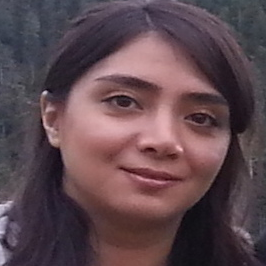
\includegraphics[width=.8\linewidth]{general_figures/forough}

\column{.5\linewidth}

\begin{block}{ALTO: Active Learning with Topic Overviews for Speeding Label Induction and Document Labeling}
Forough Poursabzi-Sangdeh, Jordan Boyd-Graber, Leah Findlater, and Kevin Seppi.  Association for Computational Linguistics, 2016.
\end{block}

\end{columns}

}

\fsi{interactive_topic_models/messy-desk}{Many Documents}

\fsi{interactive_topic_models/file-cabinet}{Sort into Categories}

\begin{frame}{Evaluation}

  \begin{itemize}
    \item User study
    \item 40 minutes
    \item Sort documents into categories
    \item What information / interface \alert<2>{helps best}
      \pause
      \pause
      \begin{itemize}
        \item Train a classifier on human examples
          \only<4->{\alert<4>{(don't tell them how many labels)}}
        \item Compare classifier labels to expert judgements
          \only<5->{\alert<5>{(purity)}}
\only<5>{
\begin{equation}
\mbox{purity}(\mathbf{U},\mathbf{G}) = \frac{1}{N}\sum\limits_{l} \max\limits_{j}|U_l \cap G_j|,
\end{equation}
}
      \end{itemize}
  \end{itemize}

\end{frame}

\begin{frame}{Which is more Useful?}

\only<1>{
  \begin{center}
    Who should drive?
  \end{center}
}


\only<2->{
\begin{columns}
  \column{.5\linewidth}
    \begin{block}{Active Learning}
      \begin{center}
        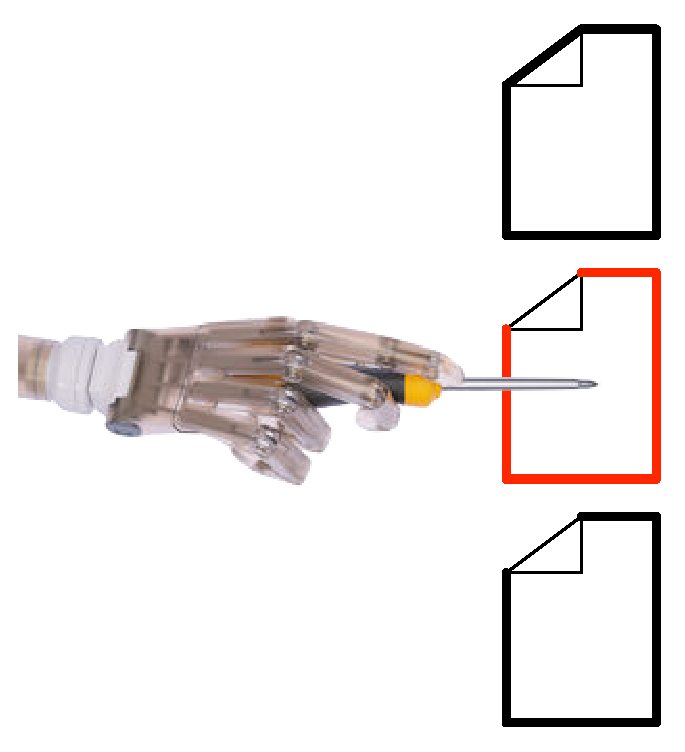
\includegraphics[width=.85\linewidth]{interactive_topic_models/active_learning}
      \end{center}
    \end{block}
  \column{.5\linewidth}
  \pause
    \begin{block}{Topic Models}
      \begin{center}
        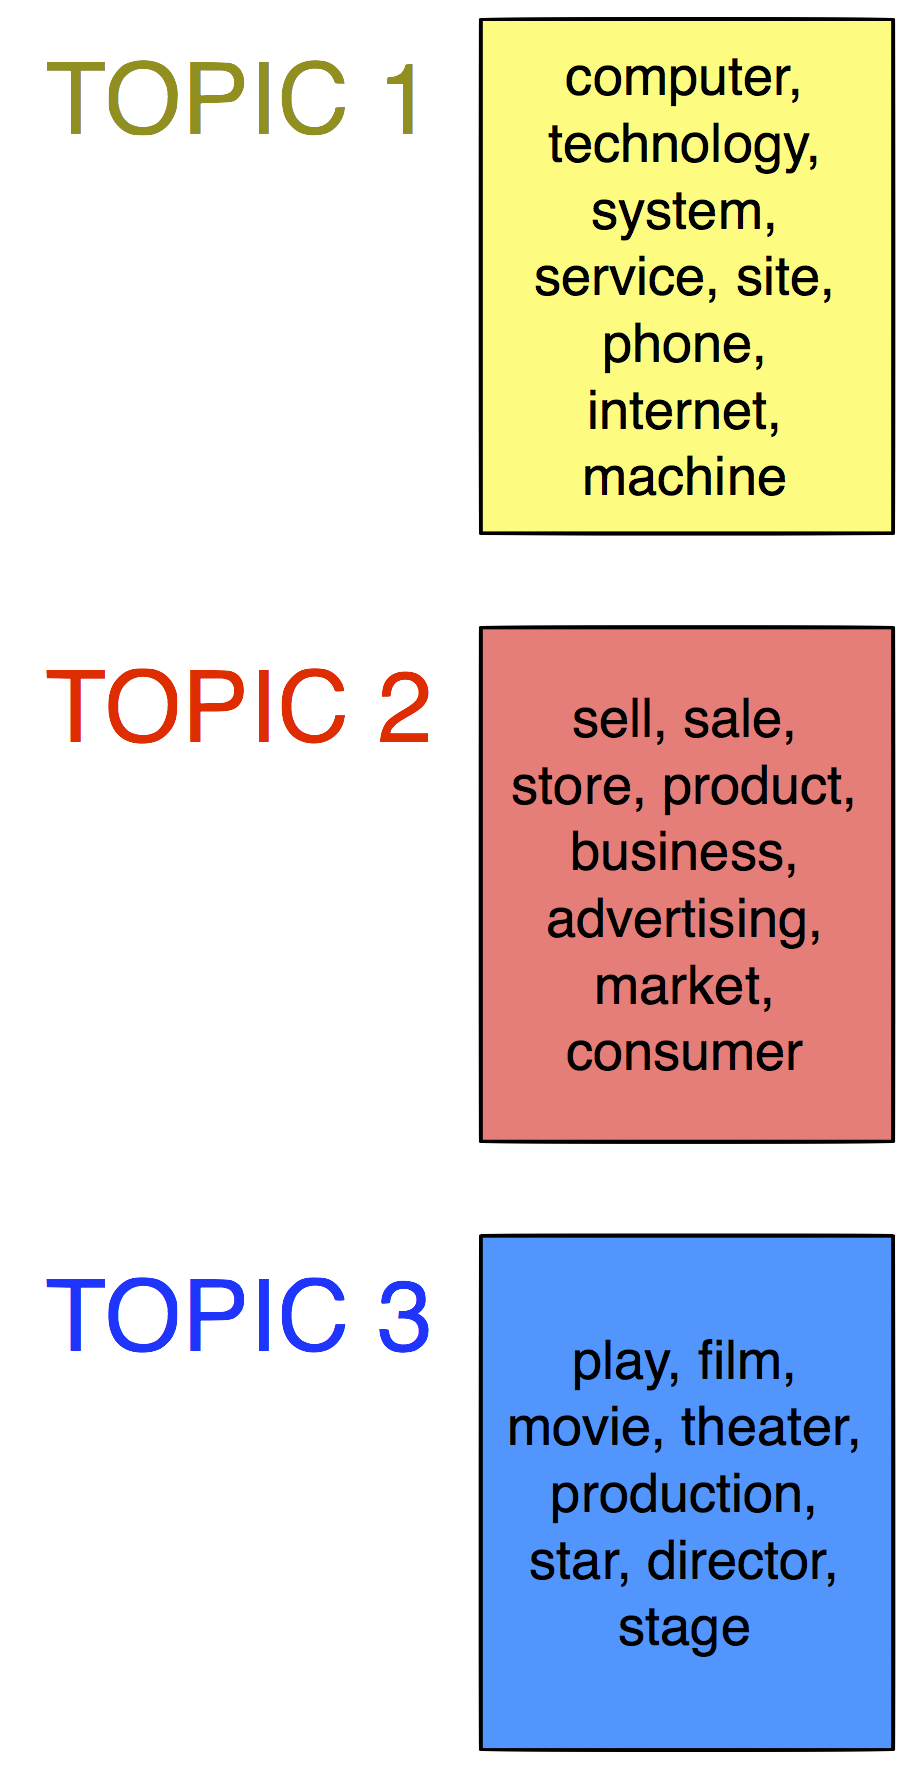
\includegraphics[width=.475\linewidth]{interactive_topic_models/nyt_topics}
      \end{center}

    \end{block}


\end{columns}
}

\end{frame}

\fsi{interactive_topic_models/alto_interface}{}
\fsi{interactive_topic_models/alto_interface_highlight}{Direct users
  to document}



\fsi{interactive_topic_models/alto/user_talk_1}{ Active learning if time is short}
\fsi{interactive_topic_models/alto/user_talk_2}{ Better than status quo}
\fsi{interactive_topic_models/alto/user_talk_3}{ Active learning can
  help topic models }
\fsi{interactive_topic_models/alto/user_talk_4}{ Topic models help
  users understand the collection }
\fsi{interactive_topic_models/alto/user_talk_4}{ Moral: machines and
  humans together (if you let them) }


\begin{frame}{What's next?}
  \begin{columns}
    \column{.45\linewidth}
    \begin{center}
      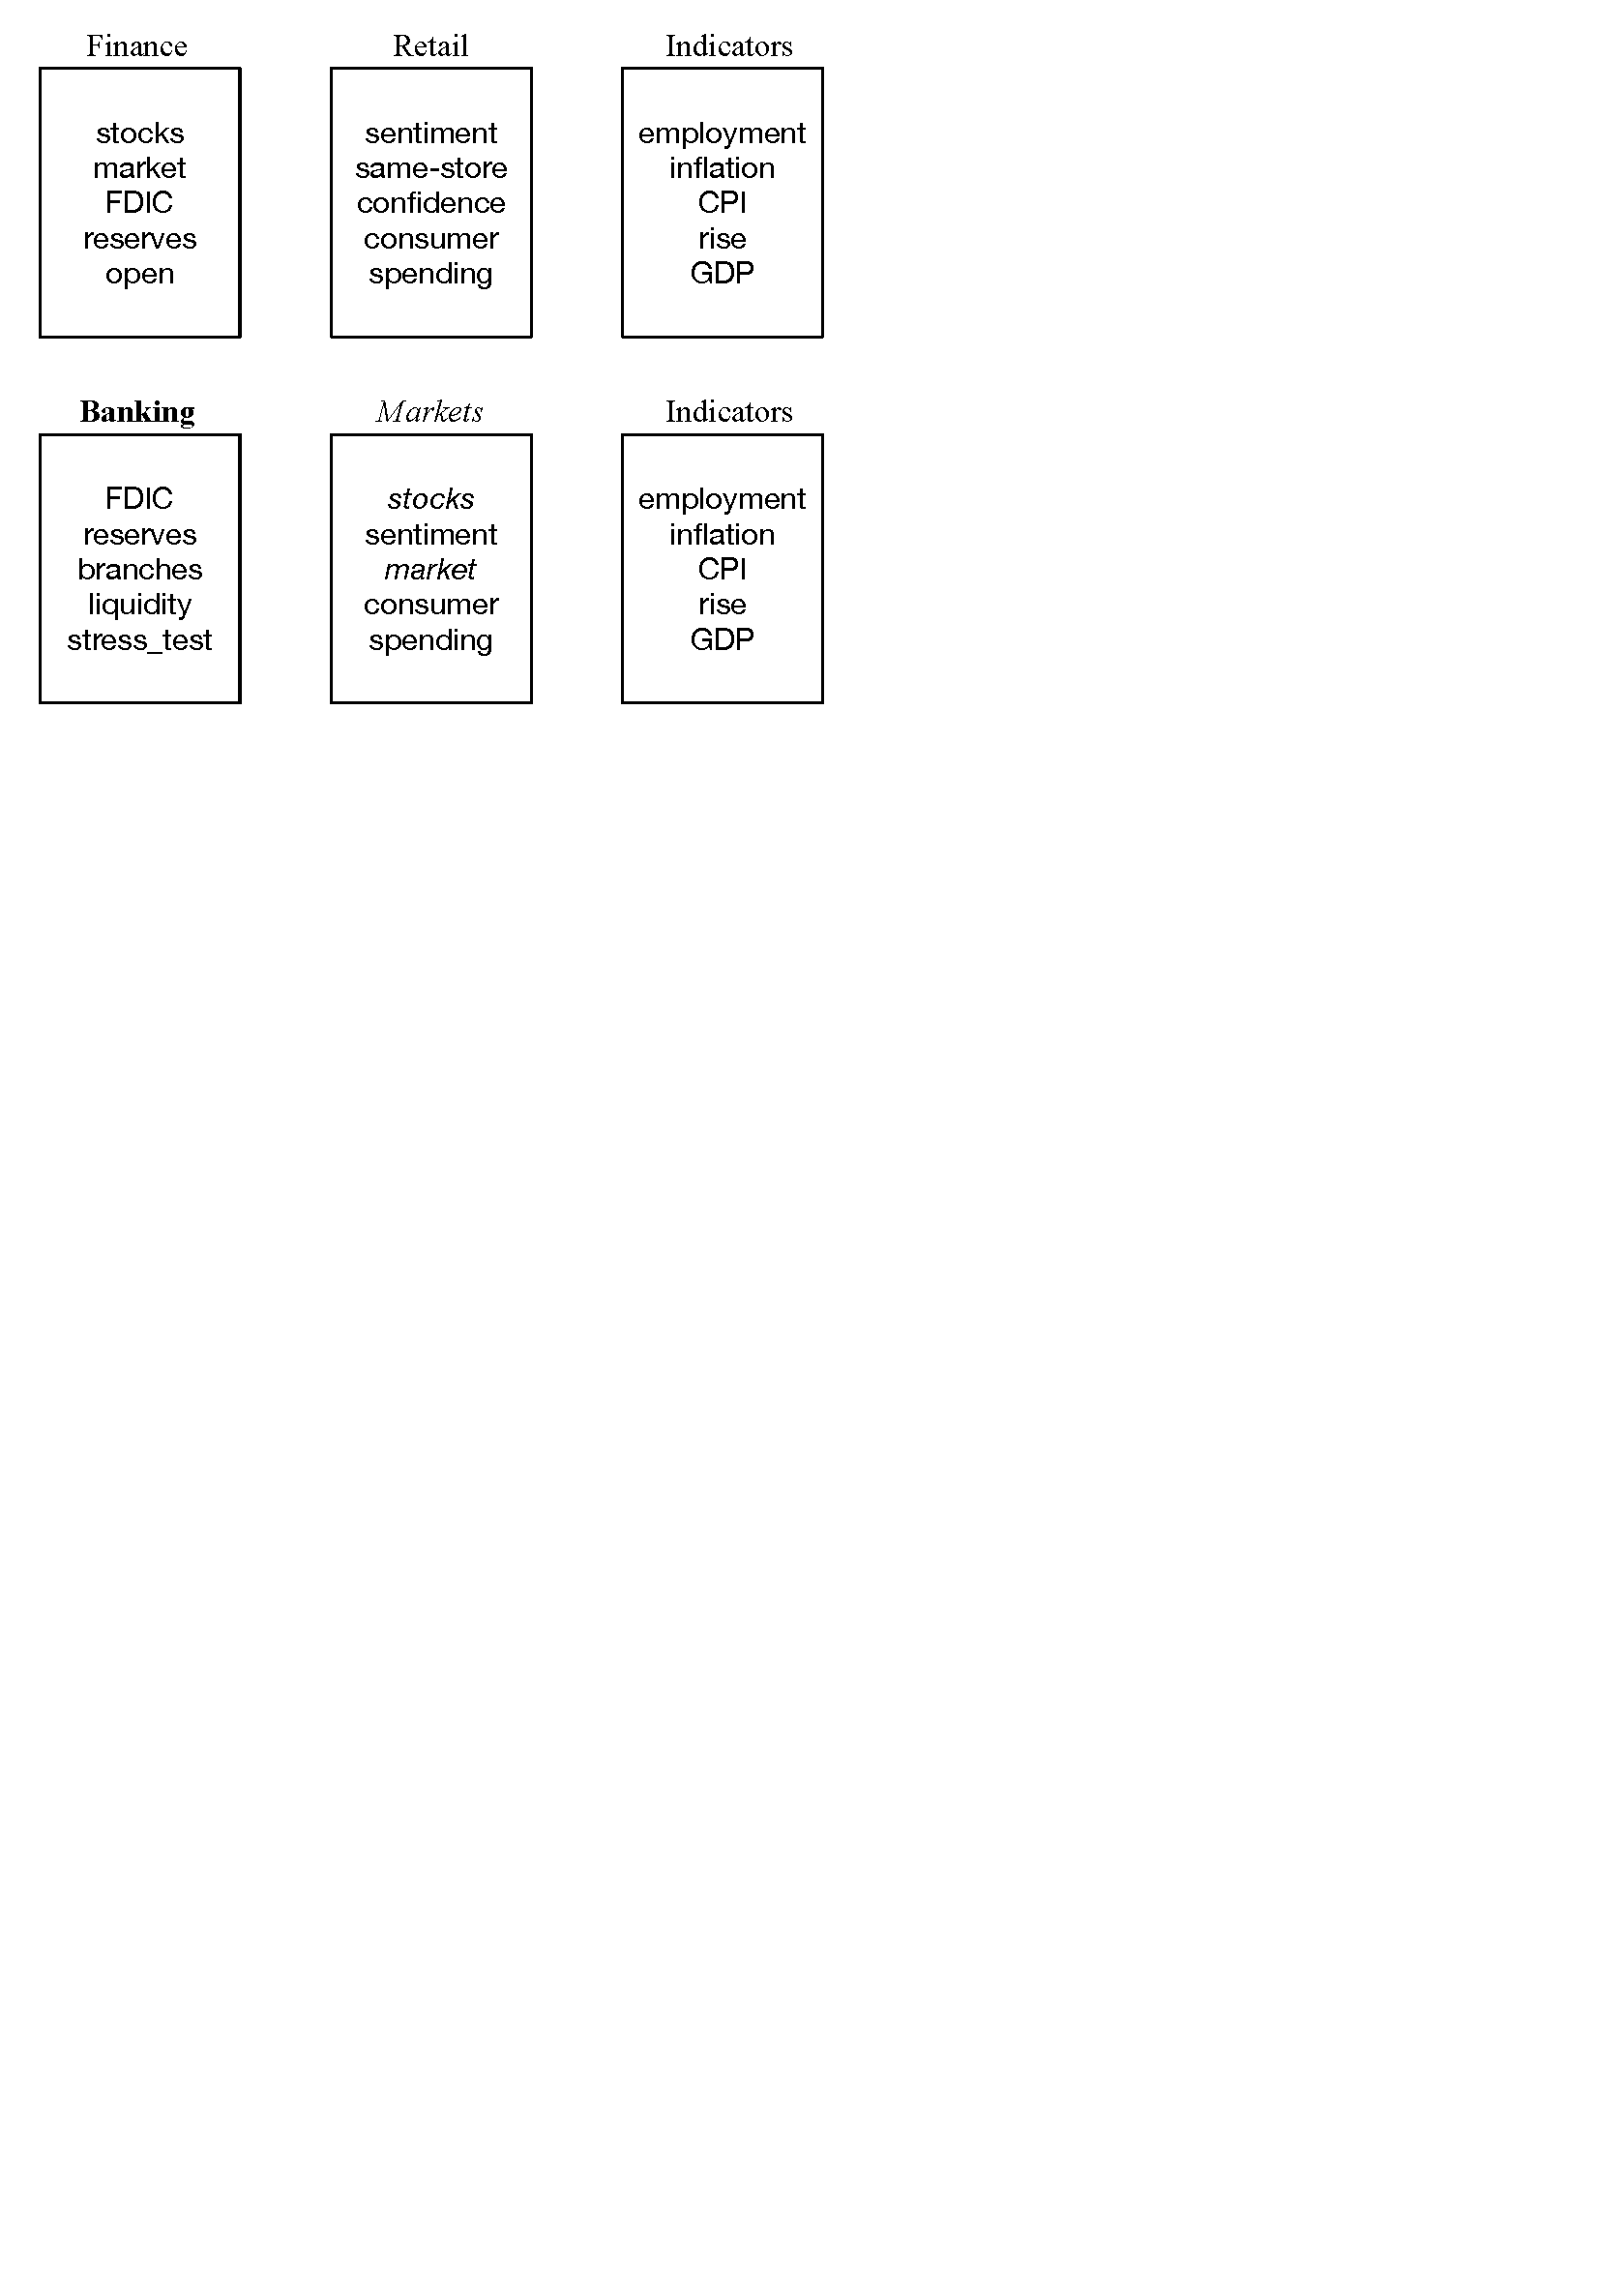
\includegraphics[width=\linewidth]{topic_models/neural_labels}
      \end{center}
     \column{.65\linewidth}
  \begin{itemize}
  \item Evaluation of whether clusterings are interpretable (neural
    models might be cheating)
  \item Automatic labeling of topic clusters
    \item Interactivity through renaming clusters: backpropagate
      through clustering
    \end{itemize}
    \end{columns}
\end{frame}


\fsi{qb/jennings_handshake}{}

\begin{frame}{Human--Computer Question Answering Competitions}
\gfxq{seattle_crowd}{.5}
\gfxq{chicago_crowd}{.5}
\end{frame}



\frame{
  \frametitle{But wait, there's more!}

  \vspace{-.5cm}

\begin{columns}



  \column{.5\linewidth}

   \begin{block}{Computational Biology}
     \centering
     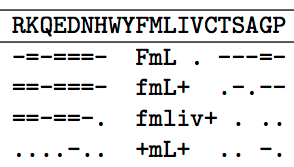
\includegraphics[width=0.4\linewidth]{general_figures/protein} \\
     \small
     \cite{nguyen-13b,hu-13:coalescent}
   \end{block}



    \begin{block}{Interactive Machine Learning}
     \centering
        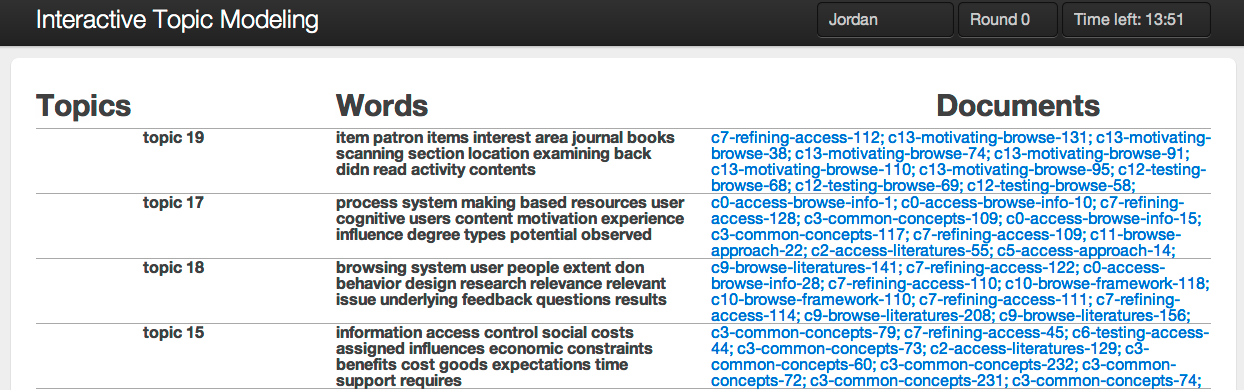
\includegraphics[width=0.4\linewidth]{interactive_topic_models/new_interface} \\
       \cite{Smith-17,Poursabzi-16}
    \end{block}


  \column{.5\linewidth}


    \begin{block}{Multilingual Analysis / Machine Translation}
      \begin{center}
        \begin{large}
          $p_{\mbox{topic}}(e | f)$ \\
         \end{large}
      \cite{eidelman-12,hu-14}
       \end{center}
    \vspace{-.3cm}
    \end{block}


    \begin{block}{Detecting Deception}
    \centering
        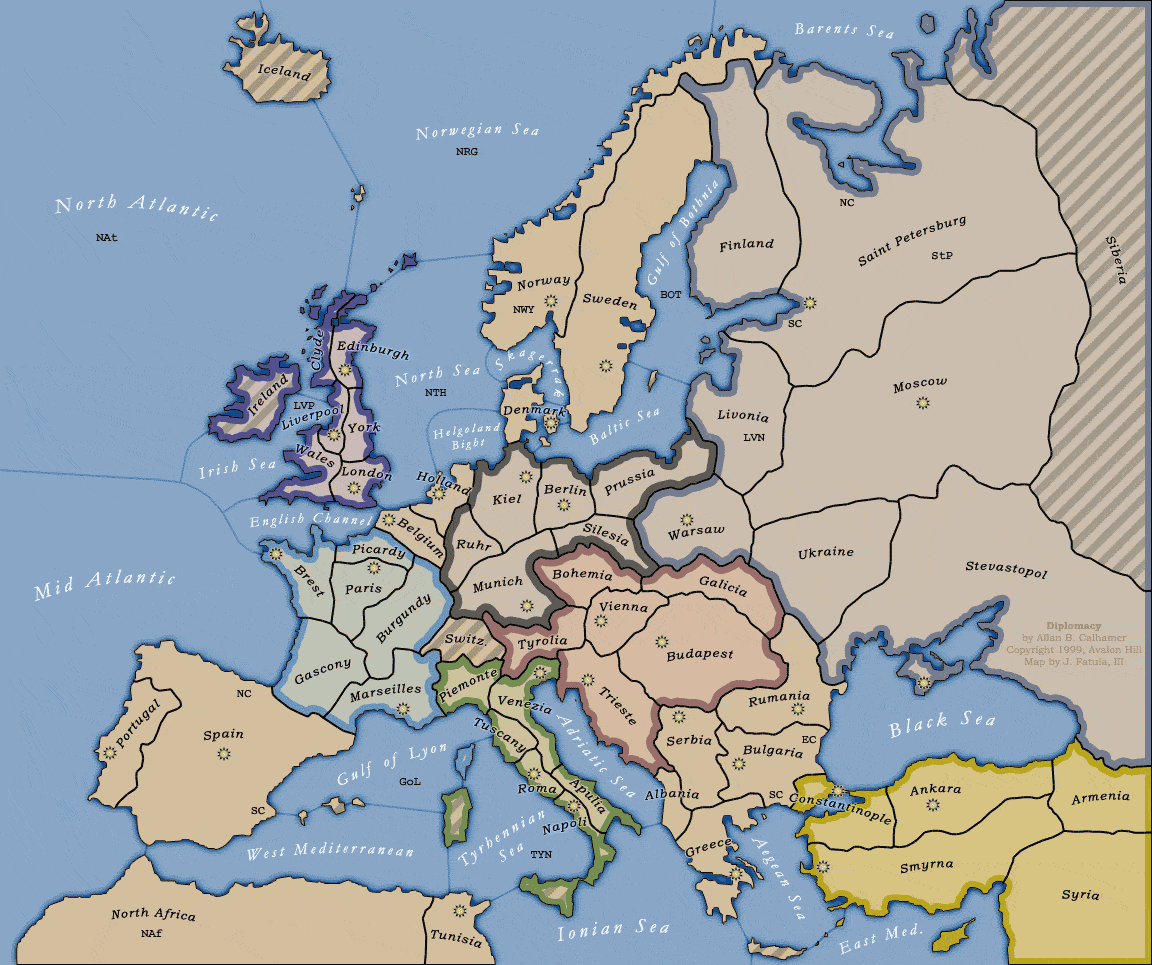
\includegraphics[width=0.4\linewidth]{general_figures/diplomacy} \\
        \cite{niculae-15,peskov-20}
    \end{block}




\end{columns}

}


\end{document}